%!TEX root = ../thesis.tex
%*******************************************************************************
%*********************************** First Chapter *****************************
%*******************************************************************************

\chapter{Introduction}  %Title of the First Chapter

\ifpdf
    \graphicspath{{Chapter1/Figs/Raster/}{Chapter1/Figs/PDF/}{Chapter1/Figs/}}
\else
    \graphicspath{{Chapter1/Figs/Vector/}{Chapter1/Figs/}}
\fi


%********************************** %First Section  **************************************
\section{Contextualisation} %Section - 1.1 

The general consensus regarding information security appears to be largely focussed on the technical aspects and approaches to implementing a holistically secure system that caters for any/all breaches \cite{Anderson2001}. One needs to consider that security within a system has to do largely with what is being protected, as well as, what malicious incentives attackers may have for wanting to gain access to information within that particular system. Incentives for attack tend to skew largely in favour of financial gain. However, another common incentive includes supporting an activist approach against organisations by gaining unauthorised access into their information systems and exposing private information to the public. As human beings our innate fear of exposure drives our motivation to protect private information that is directly/indirectly related to ourselves, our family members and/or possessions. In order to achieve this, authentication systems were developed and implemented for information systems. 

Within the security field, authentication can occur using knowledge (such as a PIN), physical possession (such as an RFID tag) and biometrics \cite{Liu2001}. Biometric information remains the most personal of possessions. By using biometric information to authenticate users the system removes problem areas such as forgotten passwords and loss of tags etc. The most basic authentication process model can be seen in Figure ~\ref{fig:basic_authentication_process_model} below.
\begin{figure}[hbtp]

\centering
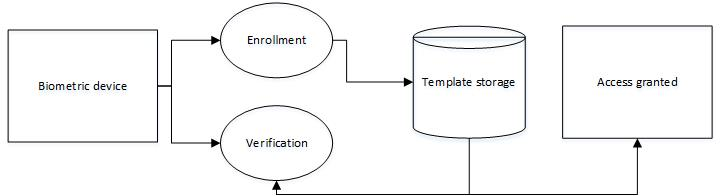
\includegraphics[width=0.8\textwidth]{Chapter1/Figs/Figure1.jpg}
\caption{ Basic authentication process model}
\label{fig:basic_authentication_process_model}
\end{figure}

The use of basic authentication systems can almost be classified as defunct, due to the fraudulent attacks becoming more commonplace. It is because of this that researchers are continuously looking for more secure forms of information protection. One of the main disadvantages of basic authentication systems is the vulnerability that occurs within storage and in transit with attackers being able to intercept sensitive authentication information at these critical points. Thus, cryptosystems were initiated. A biometric cryptosystem is an implementation technique for authenticating users by incorporating template protection (Uludag et al., 2004:948–960). One template protection scheme is known as cancelable biometrics. To classify a biometric template as cancelable, the biometric information should contain various template versions, while simultaneously being computationally irreversible. 

The concept of cryptography is predominant in steganography. Steganography is the art of surreptitiously inserting information into multimedia without changing the quality of the said multimedia (Kishor et al., 2016:1–6). This brings about the concept of combining cancelable biometrics with steganography.
The purpose of this study is to determine whether or not it is possible to improve upon biometric cancelability by using user-specific transforms, along with steganographic techniques to store biometric information.




%********************************** %Second Section  *************************************
\section{Problem Statement} %Section - 1.2


Biometrics have long been used as an accepted user authentication method and have been implemented as a security measure in many real-world systems including personal computers, mobile devices (cell phones and tablets), and physical access control (Liu \& Silverman, 2001). By encoding a person’s physical attributes the disadvantages of traditional password based security, like passwords being lost or stolen, can be overcome (Jain et al., 2016). One of the factors that hampers the acceptance of biometric authentication systems is that users have to submit private biometric data to the authentication systems and should these systems be compromised, a digital copy of their biometrics becomes available for exploitation (Rathgeb \& Uhl, 2011).

The concept of Cancelable Biometrics (CB) has to do with obfuscating of biometric information that is used for biometric authentication, whether the information is in storage or in transit. This ensures that biometric information of a person cannot be reconstructed when it is observed by a third party (Shahim et al., 2016). With the use of a cancelling technique, one can assure anonymity of users within the system and prevent unauthorised usage of digitised biometric information. One of the more common methods to ensure CB is known as biometric salting (Rathgeb \& Uhl, 2011). Biometric salting entails the introduction of random bits of data into the existing biometric information. Only when the random bits have been removed the original data can be obtained for use in a biometric system. This approach usually relies on a static salting algorithm which can be relatively easily reverse engineered (Shahim et al., 2016). Another approach to CB is presented by Dlamini et al. (2016), who posit that one can ensure the protection of user credentials in transit and in storage by using steganography to hide user information in images rather than in commonly used user databases. However, the approach of Dlamini et al. (2016) suffers from the same problem as that of biometric salting where the steganography process may be reverse engineered and biometric information can be reconstructed. 

To address these shortcomings, this study will include the incorporation of user biometric information as transform parameters for use in such a steganography engine as implemented by Dlamini et al. (2016). This results in a steganography algorithm that encodes a user’s biometric information in a picture based on their own unique traits rather than arbitrary algorithm parameters which may be computationally deduced. The premise is that each set of biometric information is stored in a different manner or location within an image and even when one user’s information is identified from the image, the fidelity of other users’ information remains intact because the transform parameters are unique to each user. This is opposed to when a common user database is breached and all the users’ information contained therein may be exposed. With the combination of steganography and CB this study can contribute to bridging the gap in biometric information storage and use within security systems.

To capture biometric information, Chan et al. (2015) presents the implementation of a Leap Motion Controller (LMC) to assume the role of a biometric authentication device. This is due to traditional biometric devices (such as fingerprint readers) having a high cost implication. The LMC is a relatively low cost input device that is usually used for motion control of computer systems. By harnessing the biometric information that is implicitly captured when the LMC is used, biometric authentication can be performed. 

Thus, this research proposes the development of a novel CB algorithm by employing a steganography approach for the storage and retrieval of biometric user information based on individual users’ physical traits where the information is obtained from an LMC. Investigation into the underlying hardware and software topics is warranted to determine the feasibility of these technological aspects before experimental implementation and testing can commence.


%********************************** % Third Section  *************************************
\section{Research question}  %Section - 1.3 
\label{section1.3}

Biometric cancelability can be enhanced using user-based transform parameters (obtained from an LMC) for a steganography algorithm that stores biometric information.


\section{Aim and objectives}  %Section - 1.4 
\label{section1.4}
The primary aim of this study is to develop a technique that ensures cancelability of biometrics based on hand geometry information from an LMC and steganographic storage techniques.
To achieve the primary objective, the following secondary objectives need to be met:

\begin{enumerate}[label=\roman*.]
\item Perform a literature study to discuss the use and implementation of cancelable biometrics, steganography, hand geometry authentication and the Leap Motion Controller.
\item Design and implementation of the system.
\item Evaluation of the created system using error-based metrics and iterative validation testing.
\end{enumerate}

\section{Research method}  %Section - 1.5 
\subsection{Introduction}
In this section various research paradigms that were considered for this study are will be discussed, followed by the chosen paradigm and research method for this study. The following research conducted on the paradigms is predominantly based on Oates (2006). The discussion entails an overview of the design science research method, preceded by a summary of both the interpretivistic and positivistic approaches.

\subsection{Interpretivistic paradigm}
\subsubsection{Introduction to interpretivism}
According to Oates(2006), interpretivism refers to the researcher’s ability to analyse an information system by means of comprehending the processes within its development in terms of social factors (Oates, 2006, p. 292). These social factors involve the people that created the systems and the dependencies from a social standpoint within a particular framework.
It can, therefore, be concluded that an interpretivistic approach to research is not focused on the proof or disproof of a particular theory. Instead, interpretivism has to do with the identification, researching techniques and the explanation of the social factors that contribute to holistically understanding a particular social context.
\subsubsection{Ontology \& epistemology}
The ontology of interpretivism has to do with being able to comprehend various kinds of opinions and interpretations in an attempt to combine multiple versions of the truth. The researcher should, thus, accept that his/her own personal perspectives and understanding of the particular topic will contribute to the final results that will be gained from the study.  This particular researcher should ensure that he/she possesses a non-neutral perspective in order to interpret the topic in a manner that is influence by the various social factors.
\subsubsection{Characteristics of interpretivistic approach}
Since interpretivism does not intend to prove or disprove a particular theory, it can be stated that once a social setting has been critically analysed a researcher has the ability to illustrate how social factors within the setting are associated and unified. Interpretivistic research paradigms have the following characteristics (Oates, 2006, p.292): 
\begin{enumerate}[label=\roman*.]
\item Realities that are subjective. The concept of ‘truth’ is based on perspectives and that one researcher's perception is likely to differ from another researcher’s, simply because of the construction of knowledge that takes place within each of our own minds.
\item Volatile construction to meaning based on social factors. Thus, the researcher is able to observe the world according to his/her own realities. Information may be subject to change in terms of context, time and culture.
\item Non-neutrality. Meaning that the researcher should maintain his/her right to make assumptions, to enforce his/her beliefs and to act upon these social factors in an attempt to conclude the research. This research is dependent on the researcher’s personal opinions.
\item Analysis of research subjects within their social settings. This means that the researcher attempts to comprehend people within their natural settings rather than creating an artificial setting. This is focused on trying to gain a perspective from the participant within that setting, as well as the observers and to merge the various perceptions using interpretation.
\item Data analysis using qualitative methods. Within the interpretivistic approach, the preferred data analysis technique is that of a qualitative nature. This involves the use of language, metaphors and imagery to gain multiple results and observations to be interpreted.
\item Numerous interpretations. Ultimately, the researcher does not expect to come to one specific conclusion, but rather combine all the extracted information and focus on the results that provide the most powerful evidence. This allows the researcher to interpret bulk amounts of information and finally concluding the study.
\end{enumerate}

\subsubsection{Interpretivistic critique}
Interpretivism involves studying social factors relating to specific social settings and behaviors within that setting. Therefore, interpretivism is an approach to research that involves multiple perspectives and relies on the above critique for the research to be viable rather than basing its credibility on the accuracy of data as a positivistic approach would.
\subsubsection{Interpretivistic methods}
The methods used within interpretivism are ethnography and case studies. Within these methods, it can be assumed that subjectivity is crucial to the research. 
\begin{enumerate}[label=\roman*.]
	\item Ethnography is successful if the researcher has the ability to successfully understand the activities of humans in interrelated cultures and to comprehend their social setting.
	\item Case studies have the focal point that ensures one specific ‘target’ is examined. This target can be analyzed in depth using various data gathering techniques.
\end{enumerate}

\subsubsection{Data gathering techniques and analysis}
Because interpretivistic researchers need to focus on the plausibility of a research topic, the data generation techniques are crucial in providing evidence for the conclusions that are drawn by the researcher. This evidence can be regarded as valid if they are generated using the following techniques (Oates, 2006, p.295):
\begin{enumerate}[label=\roman*.]
	\item Interviews;
	\item Observation;
	\item Document analysis; and
	\item Field notes.
\end{enumerate}

\subsection{Positivistic paradigm}
\subsubsection{Introduction to positivism}
According to Jokobsen, positivism refers to the positions within philosophy that accentuate both scientific methods, as well as, data that is empirical (Jokobsen, 2013). Within the Business Dictionary, positivism is a concept that perceives true knowledge to be that that is directly linked to scientific knowledge based on what is observed. It is then stated that empiricism is extended within positivism (Business Dictionary, 1999).
It can, therefore, be concluded that a positivistic approach to research is based on empiricism and the use of scientific methods to infer knowledge based on observations that are made once data has been gathered and analysed.
\subsubsection{Ontology \& epistemology}
The ontology of positivism is to do with the way in which the world is observed, measured and modelled by a specific researcher. This specific researcher should also ensure that he/she takes a neutral stand-point and is objective in his/her approach. 
With regards to epistemology in positivism, is can be stated that knowledge is classified into two basic forms. These forms include only knowledge that is empirical and knowledge that is logical (Oates, 2006).
It can be concluded that with a positivistic approach, the researcher should proceed in a neutral and objective manner while observing the world, using logic and empiricism as a guide for the conducted research.
\subsubsection{Characteristics of positivistic approach}
Because positivism is based on a ‘scientific approach’ to research, the researcher is expected to share a worldview with that of either positivistic researchers. Various assumptions can be made by these researchers that include common characteristics. According to Oates, these characteristics include the following (Oates, 2006, p. 286): 
\begin{enumerate}[label=\roman*.]
	\item Measuring and creation of models. The researcher is able to observe the world according to the positivistic ontology and using this view is able to create models of this perceived world according to the ‘facts’ obtained through scientific methods.
	\item The objective approach. The researcher should maintain impartiality as an observer throughout his/her research. This research must be independent of the researcher’s personal opinions.
	\item The testing of hypotheses. This refers to the use of empiricism within the testing of various theories or the refuting of these theories.
	\item Data analysis using quantitative methods. Within the positivistic approach, the preferred data analysis technique is that of a quantitative nature. This involves creation of mathematical models to logically and objectively analyse the given results and observations.
\end{enumerate}

\subsubsection{Positivism critique}
Because the positivism involves studying aspects relating to the natural world, researchers who prefer other methods are likely to impose on this technique. Positivism is a very general approach to research and it cannot always be used to generalize the ontology of things. This shows that there are not always predictable patterns and that research can evolve around various natural interpretations.
\subsubsection{Positivistic methods}
The method used within positivism is a scientific method. Within this method, it can be assumed that objectivity is crucial within our investigation, and that the world could be viewed as an orderly entity that does not operate in a random fashion (Oates, 2006, p. 283). 
With the use of the scientific method, it can be stated that various characteristics of positivism are used. Such characteristics include reducing problems, repeatability of processes and finally refuting theories. 
The scientific method runs through an iterative cycle which involves the following basic steps to ensure that knowledge is gained in the process:
\begin{enumerate}
	\item Create a theory from the perceived world;
	\item Instantiate an assumption or hypothesis;
	\item Use objectivity as a researcher to test the assumption;
	\item Analyse the results through observation;
	\item Use refutation or confirmation of the given assumption; and
	\item Deem the assumption accepted or rejected.
\end{enumerate}

In conclusion, the methods used within positivism are structured and involves a set process by stating the research assumption and then either accepting or rejecting the assumption based on objective observation and analysis.

\subsubsection{Data gathering techniques and analysis}
Various data gathering techniques may be used within positivistic research. Such techniques mainly involve experiments. However, other methods such as the sending out of surveys and questionnaires. Once these techniques have been used to gather data, the analysis of this data can then be described as quantitative. The second form of data analysis may be described as qualitative. This involves results obtained from interviews, observed data, narrations and documentation. Qualitative research focusses on data that is not always measurable and includes data such as textual data, images and audio when using techniques such as interviews etc. 
In conclusion, these data gathering techniques include methods such as interviews and surveys with the results being analysed in either a quantitative manner or a qualitative manner.
\subsection{Design science research}
\subsubsection{Overview}
A general definition for research would be an activity that aids in the detailed comprehension of a specific phenomenon (Vaishnavi \& Kuechler, 2015). In contrast to the aforementioned definition, DSR allows for creation of the phenomenon rather than the understanding thereof. Furthermore, research typically involves the comprehension of a phenomenon and allows the research to make some sort of prediction regarding the phenomenon’s outcome to contribute theory of knowledge that is deemed valid (based on knowledge and understanding gained throughout the process). Owen (1997) proposes that through action, knowledge can be generated. Critics occasionally consider this approach to lack in rigor. However, the process is far from unstructured.
What differentiates DSR from conventional design approaches is that it targets the unknown areas and explores the problems that may not have been solved yet. This is purely to challenge intellectual risk and to fill the void of missing knowledge within a research community (Vaishnavi \& Kuechler, 2015).
\subsubsection{DSR process model}
The DSR process model can be seen below in Figure ~\ref{fig:DSR_Process_Model} (Vaishnavi \& Kuechler, 2015). This precedes the descriptions of each of the phases in the next section.
\begin{figure}[ht]
\centering
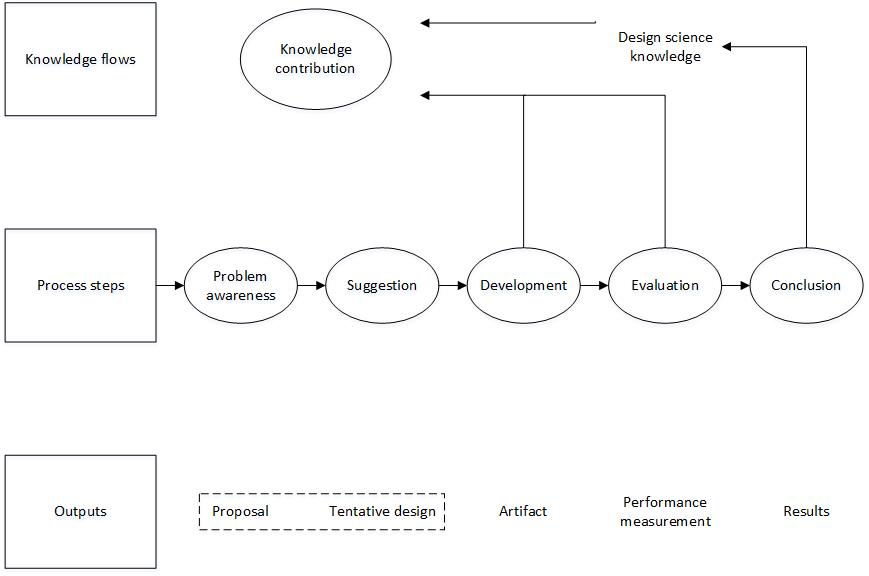
\includegraphics[width=0.8\textwidth]{Chapter1/Figs/Figure2.jpg}
\caption{DSR Process Model}
\label{fig:DSR_Process_Model}
\end{figure}

\subsubsection{Phases}
\begin{enumerate}[label=\roman*.]
	\item Awareness of the problem\\\vspace{4mm}
	To be sufficiently aware of the problem at hand it is the researcher’s responsibility to maintain constant and consistent knowledge relating to the problem from various sources (such as within allied disciplines). In this way, the researcher may come across new developments to propose improved approaches. As seen in the above figure, the output for a researcher’s awareness to a problem is ultimately a proposal.
	
	\item Suggestion \\\vspace{4mm}
	This is directly linked to the proposal as the researcher creatively displays the envisioned solution to the problem based on the awareness thereof. After having spent a considerable amount of time and effort into sufficiently comprehending the problem, if the researcher fails to produce an idea or design that suffices then the proposal will be set aside. Thus, possibly saving time that may have been spent on further research and development.
This step also cohesively ties into the positivistic approach of materialising the researcher’s curiosity relating to the phenomenon at hand.

	\item Development \\\vspace{4mm}
	The development phase merely attempts to extend upon the tentative design that was created in the suggestion phase. Implementing this phase is strongly dependent on the type of artefact to be produced. The design of the artefact may be a novelty rather than the construction thereof.
	
	\item Evaluation \\\vspace{4mm}
	Once the development of the artefact is complete, a researcher commences with evaluation thereof. This evaluation is based implicitly on criteria set out in the initial proposal. This phase is crucial to the research because any aberrations from initial anticipations must be carefully noted and thoroughly explained. It is during this phase that this positivistic approach to the problem exploration may be confirmed or acquitted. 
	
	\item Conclusion \\\vspace{4mm}
	By concluding the study, the researcher typically states whether the results sufficed the hypothesis or ‘problem exploration’ to have been accurate and justifiable by proof. These results are strengthened with knowledge gained throughout the research process and confirmed by facts observed throughout extensive studies. By concluding the study, it can be expected that a knowledge contribution be made to the specific research field.
\end{enumerate}

\subsection{Conclusion}
Upon completing the analysis of the previously discussed approaches, it was concluded that this study is positivistic in nature and should follow the DSR method. This can be motivated due to the awareness of the problem that exists within biometric authentication systems. This research intends to use that positivistic approach to verify whether or not the suggested solution will be able to enhance biometric cancelability through the development of a biometric authentication system using an LMC and steganographic techniques. Once the development of this system is complete, evaluation thereof will follow and based on the statistical data obtained, the research process can be concluded by determining whether the results justify the hypothesis.

\section{Deployment}  %Section - 1.6 
\label{section1.6}
Within Chapter 2, a literature study was conducted on related topics to the explored problem. Related research will be discussed along with the various subsections that relate to the tentative design that was created. These subsections include the concepts of biometrics, cancelability, steganography and the LMC. Furthermore, these subsections will include what each element consists of, how they work, how they suit this study and finally how they will be implemented.
In Chapter 3, the system design will be described with regards to its various elements and the chosen approach for each element will be discussed at length.
In Chapter 4, experimentation will commence by analyzing data extraction techniques, as well as testing algorithm efficiency based on extraction, processing and storing biometric information within the suggested system.
Chapter 5 will involve evaluation of the system based on implicit criteria set out within the proposal and design of the suggested model.
Finally, Chapter 6 will conclude the study by justifying the problem exploration based on results attained.

\section{Chapter summary}
\label{section1.7}
Within this chapter the basics concepts relating to this study were explained. This chapter is introductory to the purpose of the study, what the preliminary aims and objectives are and what research method will be followed. Finally, a brief over regarding the layout for the remainder of the study is given.
